\chapter{Naps}
\label{nappin}
V této kapitole rozebereme plugin pro KernelShark, se kterým budeme schopni v grafu zobrazit dobu mezi přepnutím nějaké úlohy a jejím probouzením od nějakého jiného procesu. Termínem \uv{nap} pak označujeme právě období nečinnosti nějakého procesu. V kapitole se seznámíme s cíli, analýzou řešení, návrhem a použitím tohoto pluginu. Nakonec i řešení kriticky zhodnotíme a představíme návrhy pro rozšíření.

\section{Cíle}

\begin{itemize}
    \item Mezi událostmi sched\_switch procesu P1 a sched\_waking procesu P2, který probouzí P1, se bude vykreslovat obdélník a text. Vykreslený text bude název předchozího stavu P1 před přepnutím. Vykreslený obdélník bude měnit svou barvu dle předchozího stavu.
    \item Plugin musí dostat sched\_waking události do grafů procesů, které jsou těmito událostmi probouzeny, aby mohl své grafické objekty vykreslovat.
    \item Plugin bude spolupracovat s vylepšením Couplebreak. Namísto využívání sched\_waking událostí se využijí cílové události probouzení. Spolupráce musí být automatická, tj. pokud je zapnut Couplebreak, plugin ho používá, a pokud je Couplebreak vypnutý, plugin jej nepoužívá - to vše bez vstupu od uživatele.
    \item Plugin bude možné konfigurovat skrze grafické okénko. Minimální konfigurovatelné nastavení bude maximální počet záznamů viditelných v grafu, než se plugin aktivuje. 
\end{itemize}

\section{Analýza}
Tato sekce zachytí postup postup, kterým se dostaneme k implementaci řešení. Jedná se o techničtější a detailnější analýzu než analýza z kapitoly \emph{Obecná analýza a stanovení požadavků}. Tato sekce bude často odkazovat na plugin Stacklook a jeho analýzu, abychom se vyhnuli zbytečnému opakování.

\subsection{Propojení s KernelSharkem}
Přeskočíme hlubší přemýšlení nad tím, jak připojit plugin do KernelSharku, to jsme již udělali u analýzy kapitoly pluginu Stacklook \ref{lookin-at-stacks} a stejný postup můžeme jednoduše upravit pro naše účely. V rychlosti ale zopakujeme, že plugin s KernelSharkem propojíme pomocí handlerů pro kreslení, vytváření menu nebo načítání dat. Pluginy mají kontext, ve kterém jsou proměnné pro daný plugin globální, takový kontext si sami definujeme. Implementaci propojujícího modulu rozdělíme do C kódu, který se bude starat hlavně o propojení s KernelSharkem a správné přiřazování handlerů, a do C++ kódu, který se bude starat o složitější logiku fungování pluginu.

Jediným opravu podstatným rozdílem bude handler pro načítání událostí. Nyní nebudeme pouze vybírat pro nás zajímavé záznamy událostí, kterými jsou sched\_switch a sched\_waking. Pro události typu sched\_waking je upravíme i tak, že proces, který událost vlastní, změníme z procesu probouzejícího na proces probouzený. Tím budeme pak schopni kreslit obdélníky mezi přepnutím kontextu z procesu až po jeho probouzení. Postup je velmi podobný pluginu sched\_events, který takto přesouvá pro své účely události sched\_switch.

Již zde je jasné, že pluginy si bez Couplebreaku neporadí a budou si vzájemně škodit, budou-li aktivní ve stejném streamu. V kapitole o Couplebreaku jsme sched\_events vylepšili o možnost namísto sched\_switch událostí vybírat události od Couplebreaku. Naps také bude obsahovat kód, který bude schopen Couplebreak využít. Takto bude i pěkně předvedena schopnost Couplebreaku být mostem pro kompatibilitu některých pluginů. Jediné, co my musíme přidat, je kontrola, zdali je ve streamu Couplebreak aktivován, která proběhne před určením událostí, které nás budou zajímat. Pokud je Couplebreak aktivní, tak se nebudeme zajímat o události sched\_waking, nýbrž o události sched\_waking[target]. Takto jsme stejně jako u pluginu sched\_switch odstranili nutnost měnit data trasovaných událostí a plugin žádným dalším pluginům nemůže škodit reorganizací záznamů událostí.

\subsection{Kreslení obdélníků do grafu}
KernelShark dodává API na kreslení objektů, ovšem my bychom nyní chtěli kreslit pomocí dvou záznamů v grafu, nikoli pouze pomocí jednoho, jako u Stacklooku. KernelShark má i takovou situaci vyřešenou pomocí \uv{intervalového kreslení}, tj. kreslení mezi dvěma záznamy, které přirozeně v grafu vytváří nějaký časový interval. Nám pak opět stačí jenom dodat nějakou kreslící funkci s danou signaturou, pomocí níž KernelShark obdélník nakreslí. Narozdíl od Stacklooku ale budeme kreslit obdélníky pouze v grafech procesů, jelikož doba nečinnosti procesu se zřejmě týká jenom tohoto procesu.

\subsection{Nap obdélníky}
Nyní nám už jen stačí obdélníky navrhnout. Název \uv{nap obdélník} označuje právě obdélník vytvořený tímto pluginem. Z cílů nám vychází, že musejí být dostatečně velké pro text a zároveň je dáno, že barva musí být spojena s předchozím stavem. Nejjednodušším řešením zde bude nějaká konstantní mapa předchozích stavů na barvy. Aby byly barvy jednoduše rozlišitelné, tak budeme pracovat s barvami světlými i tmavými. Přidáme ještě barvení vrchní a spodní strany obdélníku podle barvy procesu - k tomu nám pomůže dodatečné vylepšení \emph{Get Colors}. Toto barvení nebude ve výchozím nastavení zapnuto, tj. obdélníky nebudou mít žádné hrany obarvené. Cílem tohoto vedlejšího vylepšení je jak ukázka \emph{Get Colors}, tak o trochu hezčí prezentace obdélníků.

Obdélníky budou pak muset text zobrazovat dle světlosti barvy buď v černé nebo v bílé. Text umístíme někam doprostřed obdélníku. Je možné, že dva záznamy, mezi kterými má být obdélník, budou příliš blízko. Proto budeme text zobrazovat jenom pokud obdélníky budou dostatečně široké, to vypočteme pomocí délky textu k zobrazení. Podobně jako u Stacklooku získáme data pro text z informací v sched\_switch události. Nebudeme ale vytvářet samostatný mini-modul jako u Stacklooku, získání stavu bude pouze součást vytváření obdélníku.

Obdélníky nebudou mít definované interakce s uživatelem, není to součást naších cílů, tedy nebudou reagovat ani na dvojité kliknutí, ani na přejetí kurzorem myši.

\subsection{Konfigurace}
Zde využijeme dělení konfigurace ze Stacklooku na konfigurační objekt a GUI okénko, které je jediným místem pro manipulaci konfiguračního objektu. Také dáme uživateli možnost konfigurovat počet viditelných záznamů v grafu, než se plugin spustí. A podobně jako u Stacklooku přidáme zaškrtávací tlačítko pro použití funkcionalit od \emph{Get Colors}. Žádné další konfigurační možnosti nedodáme, jelikož nejsou potřeba. Pokud sestavíme Naps pro nemodifikovaný KernelShark, tak zaškrtávací políčko nebude součástí konfigurace, nemělo by pak, co měnit.

\subsection{Plugin pro nemodifikovaný KernelShark}

Stejně jako Stacklook, i Naps využije podmíněnou kompilaci pomocí makra \texttt{ifndef} s názvem \texttt{\_UNMODIFIED\_KSHARK}. Zde se bude pouze týkat barvení hran nap obdélníků.

\section{Vývojová dokumentace}

\subsection*{Dokumentace pluginu}
Dokumentace je napsána pro nástroj Doxygen. Dokumentována byla každá funkce i proměnná, ale vygenerovaná dokumentace obsahuje jen prvky veřejné. Pro implementační detaily je doporučeno se podívat do zdrojového kódu. Dokumentace obsahuje i hlavní stránku a stránku s nástinem návrhu.

\subsection*{Struktura projektového adresáře}

Adresář pluginu obsahuje další adresáře. Adresář \uv{src} je pro zdrojový kód a adresář \uv{doc} je pro dokumentaci uživatelskou a dokumentaci technickou. Očekává se, že na této úrovni jsou i adresáře pro sestavení. Na stejné úrovni žije i README, soubor s licencí a nejvyšší CMakeLists.txt. V těchto CMake instrukcích se nastaví proměnné sestavení, například typ sestavení, a případně se zavolá generování dokumentace. CMake instrukce zodpovědné za vytvoření binárního souboru jsou v adresáři se zdrojovým kódem, stejně jako to dělá KernelShark.

\subsection*{Přehled modulů pluginu}

\begin{itemize}
    \item \emph{Propojující modul} - Modul s kódem propojujícím KernelShark a plugin. Obsahem je hlavně kontext pluginu, funkce kontextu, handlery a implementačně pomocné funkce. Součástí tohoto modulu je část s C kódem a implementační část v C++ prvků z hlavičkového C souboru. Právě v \uv{C++ části} (napsaná v C++) se ostatní moduly propojují; zároveň tato část ukládá některá globální data s C++ typy. Soubory modulu jsou \emph{naps.h/c} a \emph{Naps.cpp}.
    \item \emph{Konfigurace} - Modul se skládá ze dvou tříd, konfigurační objekt a konfigurační okénko. Konfigurační objekt obsahuje konfigurační data, která plugin zrovna využívá a je navržen jako singleton. Konfigurační okénko představuje GUI element, kterým se data v konfiguračním objektu manipulují. Soubory modulu jsou \emph{NapConfig.hpp/cpp}.
    \item \emph{Nap obdélníky} - Modul se zajímá vzhled a kreslení nap obdélníků mezi záznamy. Součástí vzhledu je barva, barva vrchní a spodní hrany a text v obdélníku, tj. jeho barva, velikost a obsah. Soubory modulu jsou \emph{NapRectangle.hpp/cpp}.
\end{itemize}

\section{Uživatelská dokumentace}

Tato sekce popíše jak instalovat a používat plugin Naps v KernelSharku a co od něj během běhu očekávat, či na co si dát pozor. Malá ochutnávka fungujícího pluginu je na obrázku \ref{naps-workin}. Styl a i obsah této dokumentace jsou velmi podobné uživatelské dokumentaci Stacklooku, jelikož jsou efektivní a dají se jednoduše poupravit na jiný plugin.

\begin{figure}[p]\centering
    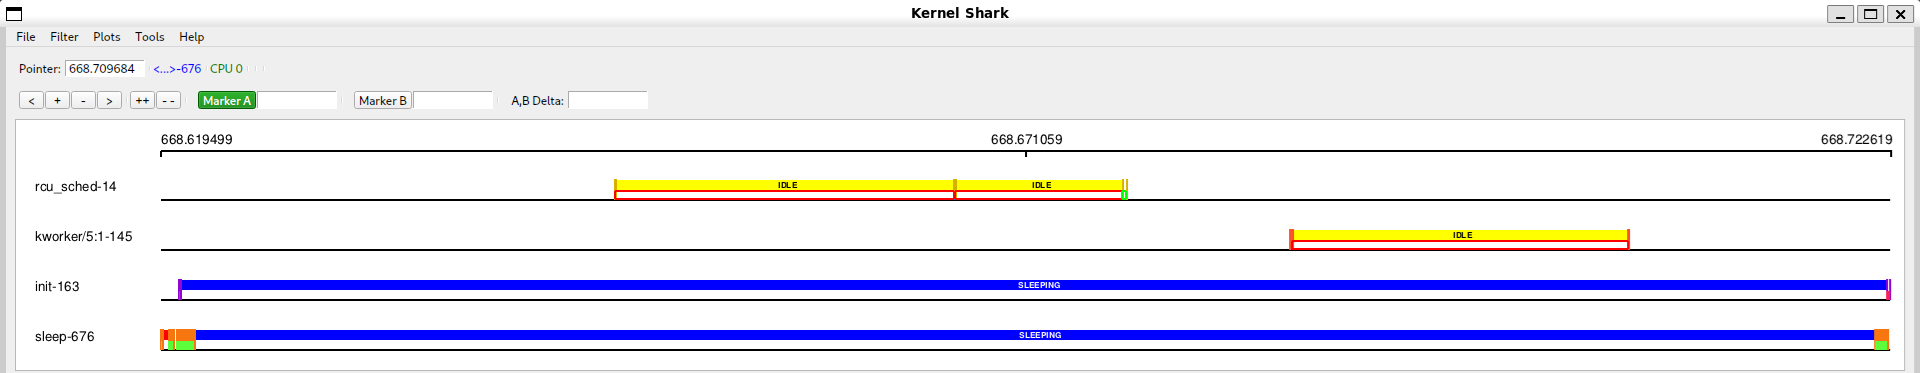
\includegraphics[width=140mm]{img/Naps/NapsWorking}
    \caption{Fungující Naps}
    \label{naps-workin}
\end{figure}

\subsection{Instalace}

\subsubsection{Předpoklady}

\begin{itemize}
  \item CMake verze alespoň 3.1.2.
  \item Pokud chceme plugin využívající modifikovaný KernelShark, pak je nutná verze alespoň 2.4.0-couplebreak. Pokud chceme plugin pro nemodifikovaný KernelShark, pak je nutná verze alespoň 2.3.2.
  \item Závislosti KernelSharku (nalezneme v README repozitáře KernelSharku), zejména Qt6 a traceevent.
  \item Doxygen na technickou dokumentaci.
\end{itemize}

Tento plugin funguje výrazně lépe, pokud je KernelShark modifikovaný. V takovém KernelSharku je plugin plně kompatibilní s oficiálními pluginy, pokud je Couplebreak zapnutý. V případě nemodifikovaného KernelSharku pak tento plugin vyžaduje vypnutí pluginu sched\_events, jinak nebude správně fungovat.

\subsubsection{Sestavení a instalace pouze pluginu}
\begin{enumerate}
  \item V terminálu nastavme pracovní adresář na složku \texttt{build} (pokud ještě neexistuje, pak ji nejlépe vytvořme v kořenovém adresáři projektu).
  \item Spusťme příkaz \texttt{cmake ..}. Pokud hlavní soubor \texttt{CMakeLists.txt} není v nadřazené složce, předejme programu CMake platnou cestu k němu.
    \begin{itemize}
      \item Používáme-li verzi KernelSharku bez modifikací, přidejme do příkazu argument \texttt{-D\_UNMODIFIED\_KSHARK}.
      Sestavení pro nemodifikovaný KernelShark odstraňuje možnost barvit vrchní a spodní hranu obdélníků kreslených pluginem barvou úlohy, které obdélník patří.
      \item Pokud chceme generovat dokumentaci pomocí Doxygenu, přidejme do příkazu argument \texttt{-D\_DOXYGEN\_DOC=1}.
      \item Výchozí typ sestavení je \texttt{RelWithDebInfo}. Chceme-li ho změnit (např. na \texttt{Release}), použijme argument \texttt{-DCMAKE\_BUILD\_TYPE=Release}.
      \item Pokud se v \texttt{/usr/include} nenacházejí hlavičkové soubory knihovny traceevent, použijme argument \texttt{-D\_TRACEEVENT\_INCLUDE\_DIR=[PATH]}, kde \texttt{[PATH]} nahradíme cestou k souborům knihovny.
      \item Pokud se v \texttt{/usr/lib64} nenacházejí sdílené objekty knihovny traceevent, použijme argument \texttt{-D\_TRACEEVENT\_LIBS\_DIR=[PATH]}, kde \texttt{[PATH]} nahradíme cestou ke sdíleným objektům knihovny.
      \item Pokud se soubory Qt6 nenacházejí ve \texttt{/usr/include/qt6}, použijme argument \texttt{-D\_QT6\_INCLUDE\_DIR=[PATH]}, kde \texttt{[PATH]} nahradíme cestou k souborům Qt6.
        \begin{itemize}
          \item Pokyny pro sestavení předpokládají, že zadaný adresář má stejnou vnitřní strukturu jako výchozí možnost (tj. obsahuje složky QtCore, QtWidgets apod.).
        \end{itemize}
      \item Pokud se zdrojové soubory KernelSharku nenachází v \texttt{../KS\_fork/src}, použijme argument \texttt{-D\_KS\_INCLUDE\_DIR=[PATH]}, kde \texttt{[PATH]} nahradíme cestou ke zdrojovým souborům KernelSharku.
      \item Pokud se sdílené knihovny KernelSharku (\texttt{.so} soubory) nenachází ve \texttt{/usr/local/lib64}, použijme \texttt{-D\_KS\_SHARED\_LIBS\_DIR=[PATH]} argument, kde \texttt{[PATH]} nahradíme cestou k sdíleným knihovnám KernelSharku.
    \end{itemize}
  \item Ve složce \texttt{build} spusťme příkaz \texttt{make}.
    \begin{itemize}
      \item Pokud je třeba sestavit jen část pluginu, například pouze dokumentaci, můžeme vybrat konkrétní cíl.
      \item Pouhé spuštění \texttt{make} vytvoří: \emph{plugin} (cíl \texttt{naps}), \emph{symlink} na sdílený objekt pluginu (cíl \texttt{naps\_symlink}) a případně \emph{Doxygen dokumentaci} (cíl \texttt{docs}), pokud tak bylo specifikováno v předchozím kroku.
    \end{itemize}
  \item (\emph{Instalace}): Nahrajme plugin do KernelSharku, buď přes GUI, nebo při spouštění přes CLI s argumentem \texttt{-p} a cestou k symlinku nebo přímo k sdílenému objektu.
    \begin{itemize}
      \item \emph{DŮLEŽITÉ}: Vždy nainstalujme/nahrajme plugin před načtením relace, ve které byl aktivní! Jinak může dojít k neúplnému načtení konfiguračního rozhraní nebo k pádu celého programu.
    \end{itemize}
\end{enumerate}

K odstranění vytvořených binárních souborů použijme \texttt{make clean}.

\subsubsection{Sestavení a instalace pomocí KernelSharku}

\begin{enumerate}
  \item Ujistěme se, že všechny zdrojové soubory (\texttt{.c}, \texttt{.cpp}, \texttt{.h}) pluginu Naps se nacházejí ve složce \texttt{src/plugins} v adresáři projektu KernelShark.
  \item Zkontrolujme, že soubor \texttt{CMakeLists.txt} v této podsložce obsahuje instrukce pro sestavení pluginu (inspirovat se můžeme podle jiných pluginů pro GUI). Pokud chceme sestavovat pro nemodifikovaný KernelShark, upravme tomu odpovídajícím způsobem build skript.
  \item Sestavme KernelShark (pluginy se sestavují automaticky). Lze sestavit i pouze plugin, pokud jsme již předtím vytvořili instrukce sestavení.
  \item (\emph{Instalace}): Spusťme KernelShark. Pluginy sestavené tímto způsobem se načítají automaticky. Pokud by se z nějakého důvodu nenačetly, najděme sdílený objekt stejně jako u ostatních oficiálních pluginů, opět buď přes GUI, nebo přes CLI.
\end{enumerate}

\subsubsection{VAROVÁNÍ - načítání více verzí pluginu}

Máme-li dvě nebo více sestavených verzí pluginu, \emph{NE}načítejme je současně do KernelSharku. Pokud to uděláme, \emph{DOJDE K PÁDU PROGRAMU}. Používejme vždy jen jednu z verzí, \emph{NIKDY OBOJE NAJEDNOU}.

\subsection{Naps v GUI}
\subsubsection{Jak zapnout Naps}

Plugin se zapíná velmi jednoduše. Stačí spustit KernelShark a přejít na položku v panelu nástrojů \texttt{Tools > Manage Plotting plugins}. Pokud byl plugin načten přes příkazový řádek, zobrazí se v seznamu pluginů jako zaškrtnuté políčko se svým názvem. Pokud ne, lze plugin dohledat pomocí tlačítka \texttt{Tools > Add plugin} - stačí nalézt symlink, ale je možné vybrat i samotný soubor sdíleného objektu. Obrázek~\ref{naps-manage-plot-plugs} ukazuje GUI pro zapínání a vypínání pluginů.

\begin{figure}[p]\centering
    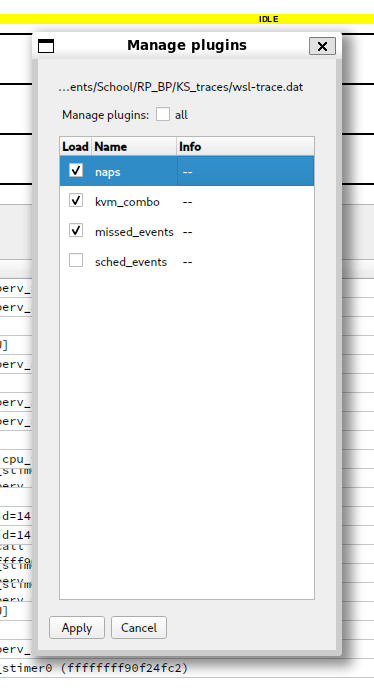
\includegraphics[height=140mm]{img/Naps/NapsManagePlottingPlugins}
    \caption{Okénko se správou pluginů se záznamem pro plugin Naps}
    \label{naps-manage-plot-plugs}
\end{figure}

\subsubsection{Konfigurace}

Konfigurace pluginu může být provedena kdykoliv, i před načtením jakýchkoliv trasovacích dat. Pro otevření konfiguračního okna (viz obrázek~\ref{naps-cfg-window}) stačí v hlavním okně zvolit \texttt{Tools > Naps Configuration}, viz obrázek \ref{naps-cfg-btn}. Vždy může být otevřeno jen jedno konfigurační okno.

\begin{figure}[p]\centering
    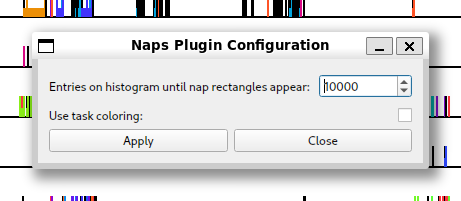
\includegraphics[width=140mm]{img/Naps/NapsConfigWindow}
    \caption{Konfigurační dialog pro plugin Naps}
    \label{naps-cfg-window}
\end{figure}

\begin{figure}[p]\centering
    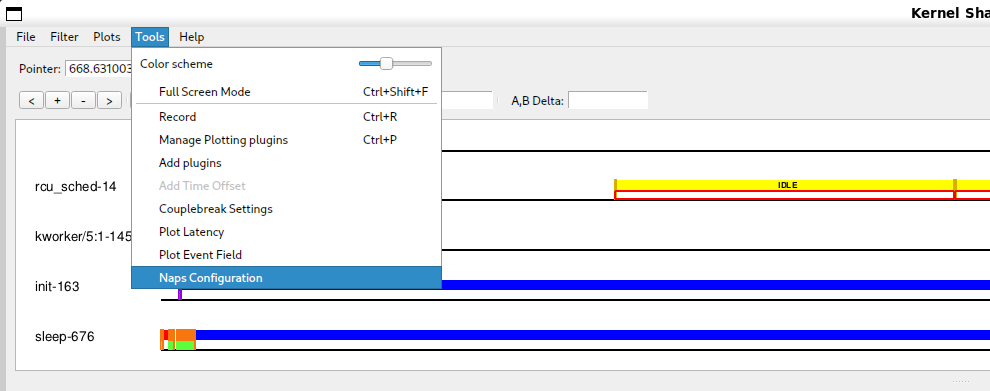
\includegraphics[width=140mm]{img/Naps/NapsConfigButton}
    \caption{Tlačítko na vyvolání konfiguračního dialogu pluginu Naps}
    \label{naps-cfg-btn}
\end{figure}

V konfiguračním dialogu lze pluginu přenastavit dvě věci. První je maximální počet viditelných záznamů v grafu trasování KernelSharku, po jehož překročení plugin nebude nic do grafu kreslit. Pokud je hodnota moc vysoká, pak dovolujeme pluginu strávit pro více událostí více času kreslením. Hodnotu je dobré snížit i tehdy, pokud pociťujeme zpomalení výkonu při kreslení s mnoha záznamy. Výchozí hodnota tohoto nastavení je 10~000 (deset tisíc) záznamů.

Druhou věcí, kterou lze konfigurovat, je barvení vrchní a spodní hrany obdélníků vykreslených pluginem barvou, kterou KernelShark využívá pro daný proces, v jehož grafu je obdélník kreslen (viz obrázek \ref{naps-task-col}). Toto se dá řídit zaškrtávacím políčkem. Ve výchozím nastavení je možnost vypnutá a je použita stejná barva, jako pro vnitřek obdélníku, viz obrázek \ref{naps-def-col}. Pokud byl ale Naps sestaven pro nemodifikovaný KernelShark, toto políčko není v konfiguraci přítomno.

\begin{figure}[p]\centering
    
\includegraphics[width=140mm]{img/Naps/NapsDefaultColors}
    \caption{Hrany obdélníku mají stejnou barvu, jako jeho vnitřek}
    \label{naps-def-col}
\end{figure}

\begin{figure}[p]\centering
    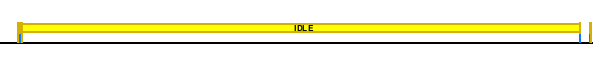
\includegraphics[width=140mm]{img/Naps/NapsTaskLikeColors}
    \caption{Hrany obdélníku používají barvu procesu}
    \label{naps-task-col}
\end{figure}

Kliknutím na tlačítko \texttt{Apply} provedené konfigurační změny potvrdíme a zavřeme tak i dialog. Zobrazí se i zpráva, že změna byla úspěšná, viz obrázek \ref{naps-cfg-succ}. Kliknutím na tlačítko \texttt{Close} nebo na křížek v hlavičce dialogu naopak změny zahodíme, ale poté také zavřeme dialog. Změny takto zahozené se při znovuotevření dialogu nevrátí, hodnoty ke konfiguraci budou stejné, jako hodnoty aktuální konfigurace.

\begin{figure}[p]\centering
    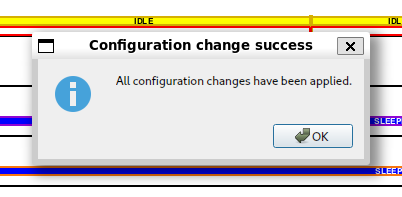
\includegraphics[width=140mm]{img/Naps/NapsConfigSuccess}
    \caption{Dialog signalizuje úspěšnou změnu konfigurace pluginu}
    \label{naps-cfg-succ}
\end{figure}

Plugin si konfiguraci nikam sám neukládá a nespolupracuje s relacemi KernelSharku. Změny provedené před zavřením programu budou muset být znovu nastaveny při dalším otevření.

\subsubsection{Naps v grafech}

Zobrazená \uv{zdřímnutí/naps} procesů jsme již viděli na začátku dokumentace. Tato sekce je trochu více představí.

K zobrazení ob nečinnosti v grafu trasování je nutné mít v tomto grafu grafy procesů. Plugin pak automaticky nakreslí barvené obdélníky mezi událostmi sched\_switch a sched\_waking/sched\_waking[target]. Barva je určena předchozím stavem procesu před přepnutím, například nepřerušitelný spánek je červený. Pokud jsme tak plugin nakonfigurovali, tak vrchní a spodní hrany obdélníků mají stejnou barvu jako proces a jeho záznamy. Pokud je obdélník dostatečně široký, tak je v něm i předchozí stav napsán velkým písmeny celým názvem. Pro příklad obdélníků s různými šířkami se podívejme na obrázek \ref{nap-diff-widths}. S obdélníky nelze nijak interagovat. Obdélníky budou viditelné tak dlouho, dokud dovolí přiblížení dvou záznamů tvořících obdélník, aby byly také viditelné.

![Fig. 8](../images/NapsDifferentWidths.png)
Figure 8.
\begin{figure}[p]\centering
    
\includegraphics[width=140mm]{img/Naps/NapsDifferentWidths}
    \caption{Obdélníky, které nejsou dostatečně široké, nezobrazí název předchozího stavu}
    \label{nap-diff-widths}
\end{figure}

Níže je seznam předchozích stavů (s anglickými názvy) a barev s nimi spjatých. Přidána jsou i krátká vysvětlení těchto stavů.
\begin{itemize}
  \item Uninterruptible (disk) sleep - červená. Proces čeká na dostupnost zdrojů a nereaguje na signály.
  \item Idle - žlutá. Pro speciální vlákno kernelu, nelze převést do stavu Running.
  \item Parked - oranžová. Pouze pro procesy kernelu, proces se dobrovolně vzdá CPU a označí se tímto stavem, aby mohl být spuštěn později. 
  \item Running - zelená. Proces běží na nějakém CPU.
  \item Sleeping - modrá. Proces čeká na dostupnost zdrojů a reaguje na signály.
  \item Stopped - azurová. Procesu byl zaslán STOP signál.
  \item Tracing stop - hnědá. Proces se zastavil, jelikož je právě trasován či laděn.
  \item Dead - magenta/purpurová. Přechodný stav těsně předtím, než bude proces dealokován.
  \item Zombie - fialová. Proces skončil svou práci a čeká na uklizení rodičovským procesem.
\end{itemize}

\subsection{Bugy a chyby}

Žádné nejsou známy.

\subsection{Doporučení}

Autor níže vypisuje pár doporučení při používání pluginu.
\begin{itemize}
  \item Vždy načtěme Naps před načtením relace. Může to programu ušetřit nepříjemná překvapení.
  \item Pokud chceme dvě verze pluginu, sestavme je do různých adresářů.
  \item Opakujeme, že je doporučeno používat verzi pluginu s KernelSharkem, který obsahuje Couplebreak.
  \item Nedoporučuje se nastavovat příliš vysoký limit záznamů v grafu v konfiguraci. Jinak by plugin mohl používat příliš mnoho paměti kvůli velkému množství naráz kreslených nap obdélníků.
  \item I když relace v KernelSharku fungují, jsou trochu nestabilní. Tento plugin se snaží jejich vnitřní logiku nenarušovat, ale varuje, že pokud plugin není načten předem, mohou nastat neočekávané problémy. Například načtení relace s aktivním pluginem nepřidá do menu \texttt{Tools} odpovídající položku pro vyvolání konfiguračního okna.
\end{itemize}

\section{Rozšíření}
\subsubsection*{Interakce}
Obdélníky fungují dobře, ale možná by bylo dobré přidat nějakou interakci, která by nám o době nečinnosti dala další informace. Například by při přejetí myši mohl informační řádek KernelSharku, nebo nějaká plovoucí vysvětlivka ukázat i rozdíl mezi časem přepnutím a probouzením. Nebo by mohlo být při dvojitém kliknutí zobrazeno okénko, ve kterém jsou nějaké statistiky a detaily o době nečinnosti. Přímé rozšíření tedy nedodáváme, ale tato nastínění snad ukazují, že rozšířit tento jednoduchý plugin lze.

\subsubsection*{Persistentní konfigurace}
Stejně jako u Stacklooku, i zde by bylo pěkné mít schopnost ukládat si konfiguraci z nějaké relace KernelSharku. Zde je problém trochu mírnější, jelikož máme méně věcí, co lze konfigurovat. Ale i tak by bylo lepší nemuset při každém otevření KernelSharku a načtení pluginu manuálně konfiguraci měnit.

\section{Kritika}
Plugin je vcelku malý a autorovi se zdá, že funguje docela bezproblémově. Tu kritiku, kterou má, sdílí se Stacklookem, tj. \emph{Konfigurační singleton} a \emph{Verze pluginu pro nemodifikovaný KernelShark}. I zde platí ty stejné argumenty jako pro Stacklook.

\section{Zhodnocení splnění požadavků}
Plugin zřejmě splňuje první z obecných cíle pluginů, tj. vlastní adresář s instrukcemi k sestavení. Nezávislost na jiných pluginech není dokonale splněna, pokud plugin neběží v prostředí s Couplebreakem. Pokud tomu tak není, tak si s pluginem sched\_events vzájemně škodí a jsou tak na sobě závislé tak, že se vzájemně zakazují. Tomu se bohužel nedá předejít, jelikož není jiný způsob, jak by každý z nich dokázal odvést svou práci.

Jinak jsme v analýze postupovali tak, abychom každý z našich cílů splnili. Navíc jsme nepřišli na žádné další problémy při vytváření řešení. Tím jsme splnili i požadavky vlastní.